%
% Schwarze Löcher
%
\section{Schwarze Löcher und die Schwarzschild-Metrik
\label{buch:kruemmung:section:schwarzesloch}}
\kopfrechts{Schwarze Löcher und die Schwarzschild-Metrik}
Mit der Aufstellung der Feldgleichungen stellt sich sofort die Frage
nach Lösungen derselben.
Da die Feldgleichungen nichtlineare partielle Differentialgleichungen
zweiter Ordnung sind ist nicht zu erwarten, dass Lösungen ohne
zusätzliche Annahmen leicht zu finden sind.

%
% Die Schwarzschild-Metrik
%
\subsection{Die Schwarzschild-Metrik}
Eine naheliegende vereinfachende Annahme ist das Gravitationsfeld
eines kugelsymmetrischen Körpers, zum Beispiel eines nicht oder nur
sehr langsam rotierenden und zeitlich unveränderlichen Sterns.
Der Kugelsymmetrie mit mit dem Ursprung im Mittelpunkt des Sterns
tragen die Kugelkoordinaten $(r,\vartheta,\varphi)$ im Raum Rechnung.
Die Metrik darf in diesem Fall nur von der $r$-Koordinate abhängen.

Bereits einen Monat nach der Veröffentlichung von Einsteins Arbeit
über die allgemeine Relativitätstheorie hat Karl Schwarzschild
\index{Schwarzschild, Karl}%
die Lösung
\begin{equation}
ds^2
=
\biggl( 1-\frac{r_s}{r} \biggr)
c^2\,dt^2
-
\biggl(1-\frac{r_s}{r}\biggr)^{-1}
\,dr^2
-r^2 (d\vartheta^2 + \sin^2\vartheta\,d\varphi^2),
\label{buch:kruemmung:blackhole:eqn:schwarzschild}
\end{equation}
die sogenannte \emph{Schwarzschild-Metrik}
\index{Schwarzschild-Metrik}%
gefunden.
Die Koordinatenlinien sind orthogonal, da die ausserdiagonalen Elemente
des metrischen Tensors in diesen Koordinaten verschwinden.
Die Determinante der Metrik ist
\begin{equation}
-g
=
\biggl( 1-\frac{r_s}{r} \biggr)
c^2
\biggl(1-\frac{r_s}{r}\biggr)^{-1}
r^4 \sin^2\vartheta
=
c^2r^4\sin^2\vartheta,
\label{buch:kruemmung:schwarzesloch:eqn:g}
\end{equation}
stimmt also mit dem Wert der euklidischen Metrik in diesen Koordinaten
überein.

%
% Krümmung
%
\subsection{Krümmung}
Die einsteinschen Feldgleichungen verknüpfen die Masseverteilung mit
der Krümmung.
Die Berechnung der Ricci-Krümmung und des Krümmungsskalars ergibt
für beide $0$.
Die Schwarzschild-Metrik beschreibt also das Vakuum um den Nullpunkt,
nicht die Situtation im Nullpunkt selbst.

Dies bedeutet jedoch nicht, dass das Feld keine Gravitationswirkung
beschreibt.
Für die Berechnung der Geodäten, die nahe am räumlichen
Nullpunkt vorbeiführen, müssen die Zusammenhangskoeffizienten
bestimmt werden, was einigermassen aufwendig ist und hier nicht
durchgeführt wird.
Der Vergleich mit der newtonschen Approximation von
Abschnitt~\ref{buch:kruemmung:section:newton}
zeigt aber, dass der von $1$ abweichende Wert von $g_{tt}$ auf
eine Gravitationswirkung hinweist.
Es muss also eine Masse geben, die mit der beobachteten Gravitationswirkung
assoziiert werden kann.

%
% Der Schwarzschild-Radius
%
\subsection{Der Schwarzschild-Radius}
%
% table-schwarzschildradius.tex
%
% (c) 2025 Prof Dr Andreas Müller
%
\begin{table}
\centering
\begin{tabular}{|l|>{$}r<{$}|>{$}r<{$}|>{$}r<{$}|}
\hline
Objekt & R\,\textrm[m]& M\,\textrm{[kg]}&r_s\raisebox{3pt}{\strut}\\[2pt]
\hline
Fussball
	& 0.011\phantom{\mathstrut\cdot 10^{22}}
	& 0.450\phantom{\mathstrut\cdot 10^{22}}
	& 6.684\cdot{10^{-28}}\rlap{$\,\mathrm{m}$}\hspace*{6mm}
\raisebox{5pt}{\mathstrut}
\\
Mond
	& 1.737\cdot 10^{6\phantom{0}}
	& 7.346\cdot 10^{22}
	& 0.011\rlap{$\,\mathrm{mm}$}\hspace*{6mm}
\\
Erde 
	& 6.378\cdot 10^{6\phantom{0}}
	& 5.972\cdot 10^{24}
	& 8.870\rlap{$\,\mathrm{mm}$}\hspace*{6mm}
\\
Jupiter
	& 1.429\cdot 10^{8\phantom{0}}
	& 1.898\cdot 10^{27}
	& 2.829\rlap{$\,\mathrm{m}$}\hspace*{6mm}
\\
Sonne
	& R_{\sun}=6.963\cdot 10^{8\phantom{0}}
	& M_{\sun}=1.988\cdot 10^{30}
	&2.952\rlap{$\,\mathrm{km}$}\hspace*{6mm}
\\
Polarstern
	& 46.27\,R_{\sun}
	& 5.13\,M_{\sun}
	& 15.1\phantom{00}\rlap{$\,\mathrm{km}$}\hspace*{6mm}
\\
VY Canis Maioris
	& 1420\phantom{.00}\,R_{\sun}
	& 17\,M_{\sun}
	& 40.2\phantom{00}\rlap{$\,\mathrm{km}$}\hspace*{6mm}
\\
PSR J1748-2446ad
	& 16\cdot10^{3\phantom{0}}
	& 2\phantom{.00}\,M_{\sun}
	&  6\phantom{.000}\rlap{$\,\mathrm{km}$}\hspace*{6mm}
\\
Stellares SL
	&
	& 10\phantom{.00}\,M_{\sun}
	&  29.52\phantom{0}\rlap{$\,\mathrm{km}$}\hspace*{6mm}
\\
Supermassives SL
	&
	& 10^5\text{--}10\rlap{$\mathstrut^{11}$}\phantom{.00}\,M_{\sun}
	&   0.002\text{--}2000\rlap{$\,\mathrm{AU}$}\hspace*{6mm}
\\[2pt]
\hline
\end{tabular}
\caption{Schwarzschild-Radien einer Objekte des Sonnensystems und
einiger schwarzer Löcher.
VY Canis Maioris ist der grösste bekannte Stern. PSR J1748-2446d ist
der Pulsar mit der schnellsten bekannten Rotation.
Stellare schwarze Löcher (SL) entstehen beim Kollaps eines Sterns
am Ende seines Lebens, während supermassive SL im Zentrum von
Galaxien zu finden sind.
Eine Astronomische Einheit (AU) ist die mittlere Entfernung zwischen
Sonne und Erde und beträgt $1.495978707\cdot 10^8\,\text{km}$.
\label{buch:kruemmung:schwarzesloch:table:schwarzschildradien}}
\end{table}
%
Die Konstante $r_s$ heisst \emph{Schwarzschild-Radius}.
\index{Schwarzschild-Radius}%
Für grosse Werte $r\ll r_s$ kann der Quotient $r_s/r$ vernachlässigt
werden und \eqref{buch:kruemmung:blackhole:eqn:schwarzschild} geht
in die Minkowski-Metrik über.

Für weniger grosse Entfernungen erwartet man, dass die beobachtete
Wirkung mit der einer weit entfernten Punktmassen übereinstimmt.
Die newtonsche Approximation stellt einen Zusammenhang zwischen
dem Gravitionspotential und dem Koeffizienten her.
Nach \eqref{buch:kruemmung:newton:eqn:metrik} ist
\[
g_{00} = 1+\frac{2U(x)}{c^2}.
\]
Durch Vergleich mit der Schwarzschild-Metrik
\eqref{buch:kruemmung:blackhole:eqn:schwarzschild}
kommen wir zur Approximation
\[
1
+
\frac{2U}{c^2}
=
1
-
\frac{r_s}{r}
\qquad\Rightarrow\qquad
r_s
=
-
\frac{2Ur}{c^2}.
\]
Das newtonsche Gravitationspotential einer Masse $M$ ist $U=-GM/r$,
somit wird der Schwarzschild-Radius zu
\[
r_s
=
\frac{2GM}{c^2}.
\]

Für Radiuswerte, die im Vergleich zum Schwarzschild-Radius klein sein,
spielen die relativistischen Effekte eine untergeordnete Rolle.
Die Objekte in Sonnennähe haben vergleichsweise kleine Masse und damit
ist auch der zugehörige Schwarzschild-Radius sehr klein.
Die Tabelle~\ref{buch:kruemmung:schwarzesloch:table:schwarzschildradien}
stellt die Schwarzschild-Radien einiger vertrauter Objekte zusammen.
Die Objekte des Sonnensystems sind um viele Grössenordnungen grösser
als ihr Schwarzschild-Radius, selbst für die Sonne ist der
Schwarzschild-Radius nur etwa 3\,km, daher bedarf es besonderer 
Anstrengung, die Effekte der allgemeinen Relativitätstheorie überhaupt
zu messen.
\index{Rsonne@$R_{\sun}$}%
\index{Msonne@$M_{\sun}$}%
Die Lichtablenkung durch die Gravitation der Sonne macht nur etwa
$2''$ aus, sie erfolgt ungefähr $2R_{\sun}$ von der Sonne entfernt.
Die Drehung der Apsidenlinie der Merkurbahn macht $42.98''$ pro
Jahrhundert aus, dies ist eine Wirkung in der Entfernung des
Merkurbahnradius von der Sonne, was etwa $83R_{\sun}$ entspricht.
Für die weiter entfernten Planeten ist die Periheldrehung um Grössenordnungen
kleiner.

%
% Der Ereignishorizont
%
\subsection{Der Ereignishorizont}
Bei Annäherung an $r=r_s$ geht der Term $r_s/r$ gegen $1$, entsprechend
divergiert der Koeffizient von $dr^2$,
das verwendete Koordinatensystem ist also ungeeignet.
Da die Determinante \eqref{buch:kruemmung:schwarzesloch:eqn:g}
der Metrik bei $r=r_s$ weder gegen $0$ noch
gegen $\infty$ geht, ist aber nicht mit einer wirklichen
Singularität bei $r=r_s$ zu rechnen.
Tatsächlich kann man in den sogenanten Finkelstein-Koordinaten
einen Ausdruck für die Metrik finden, die das Problem nicht hat.

Für ein Teilchen, welches sich näher als bei $r=r_s$ am Objekt
vorbeibewegt, ändert plötzlich das Vorzeichen des $dt^2$-Terms.
Es muss also einen grundlegenden Unterschied in den Bereichen
$r>r_s$ und $r<r_s$ geben.

Für $r>r_s$ wird der Lichtkegel durch die Linien gegeben, für
die die Metrik den Wert 0 ergibt.
\index{Lichtkegel}%
Aus \eqref{buch:kruemmung:blackhole:eqn:schwarzschild} liest man
ab, dass 
\[
\biggl(1-\frac{r_s}{r}\biggr) c^2\, dt^2
=
\biggl(1-\frac{r_s}{r}\biggr)^{-1}\,dr^2
\qquad\Rightarrow\qquad
\frac1c\frac{dr}{dt}
=
\pm
\biggl(1-\frac{r_s}{r}\biggr)
\]
sein muss.
%
% fig-sl.tex
%
% (c) 2025 Prof Dr Andreas Müller
%
\begin{figure}
\centering
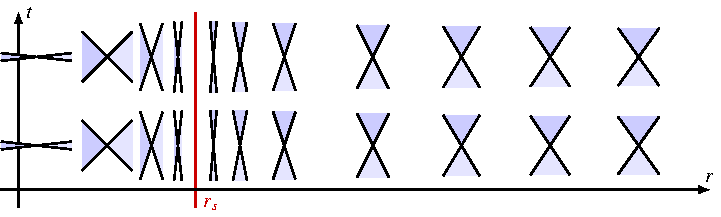
\includegraphics{chapters/110-kruemmung/images/sl.pdf}
\caption{Entstehung des Ereignishorizontes bei einem schwarzen Loch.
Ausser von $r=r_s$ 
Innerhalb $r=r_s$ ist die Richtung der Zukunft ausschliesslich zu
abnehmenden Werten von $r$ gerichtet.
Teilchen können sich also nur noch auf Bahnen bewegen, die innerhalb
$r_S$ bleiben.
\label{buch:kruemmung:schwarzesloch:fig:sl}}
\end{figure}

%
In einem $r$-$ct$-Diagramm entspricht das zwei Linien, die
in einem Winkel 
\[
\alpha = \arctan \biggl(1-\frac{r_s}{r}\biggr)
\]
zur $r$-Achse stehen.
Die beiden Richtungen sind in
Abbildung~\ref{buch:kruemmung:schwarzesloch:fig:sl}
durch schwarze Linien angezeigt.

Der Bereich der Zukunft oder Verangenheit von einem Weltpunkt aus
wird durch negative Werte der Metrik angezeigt.
Für $r>r_s$ ist dies der Bereich zwischen den beiden Strahlen in
$t$-Richtung.
Für $r<r_s$ kehrt jedoch das Vorzeichen der Metrik, der Kegel der
Zukunft zeigt jetzt in Richtung abnehmender $r$.
In Abbildung~\ref{buch:kruemmung:schwarzesloch:fig:sl} ist die
Zukunft durch ein blaues Dreieck angezeigt, die Vergangenheit durch
helleres Blau.
Dies bedeutet, dass ein Teilchen nach dem Überschreiten der Grenze $r=r_s$
sich nur noch in Richtung abnehmender $r$ bewegen kann, die Zukunft des
Teilchens befindet sich vollständig innerhalb $r_s$.

Aus dem Bereich $r_s$ gibt es also kein Entkommen, nicht einmal
für Lichtstrahlen.
Man sagt, bei $r_s$ befinde sich der \emph{Ereignishorizont}.
\index{Ereignishorizont}%
Ein Objekt mit einem Radius, der kleiner ist als sein Schwarzschild-Radius
wird daher als \emph{schwarzes Loch} bezeichnet.
\index{schwarzes Loch}%
Von aussen gibt es keine Möglichkeit, irgend etwas darüber zu sagen,
was innerhalb des Schwarzschild-Radius passiert.

%
% Rotierende Objekte und die Kerr-Metrik
%
\subsection{Rotierende Objekte und die Kerr-Metrik}
Übliche Modelle der Sternentstehung zeigen allerdings, dass es fast
unmöglich ist, dass ein Objekt von der Grösse eines Sterns keinen 
verbleibenden Drehimpuls hat.
Noch dramatischer wird die Situation bei Neutronensternen, wo 
Rotationsfrequenzen von bis zu $716\,\text{Hz}$ gemessen worden sind.
Da Neutronensterne auch sehr hohe Masse bei kleinen Abmessungen
aufweisen, kann nur die allgemeine Relativitätstheorie das Gravitationsfeld
adäquat beschreiben.
Eine Lösung ist die von Roy Kerr gefundene \emph{Kerr-Metrik},
die aber hier nicht weiter diskutiert wird.
\index{Kerr, Roy}%
\index{Kerr-Metrik}%

